\documentclass{resume}
\name{Eric Kim}
\addressone{2246 8th Street, A}
\addresstwo{Berkeley, CA 94710}
\email{eric.kim.cs@gmail.com}
\phone{805-300-9474}
\website{http://www.eric-kim.net}

\usepackage{verbatim}
\usepackage{graphicx}

\begin{document}

\maketitle
\thispagestyle{empty} %% no page numbers

\begin{component}{About Me}
I am a recent Berkeley graduate interested in pursuing a PhD degree in Computer 
Science.

As an undergraduate, I quickly developed a keen interest in the field, 
and earnestly devoted myself to my studies. Wishing to examine the 
material at a deeper level, I pursued several 
teaching opportunities for a variety of undergraduate CS courses. My
most significant (and memorable) teaching experiences have occured while 
TA-ing the undergraduate CS 61A course, with both Brian Harvey and John
DeNero as instructors. Under Brian Harvey, I refined my teaching style, and
was greatly influenced by the positive learning environment encouraged by
Brian and reciprocated by the students. Later, with John DeNero, I participated
in developing the ``new'' 61A, taught in Python, where I helped develop
course materials such as discussion notes and exams.
Through these valuable teaching 
experiences, I developed a strong interest in teaching that I wish to
continue to nurture.

In addition, my desire to learn more about the CS field led me to
work with Professor David Wagner's ``Electronic Voting and Computer Vision''
research group, where we developed several tools and performed pilot audits
with various California counties, in addition to publishing at EVT/WOTE. Our major
contributions are systems in which Computer Vision algorithms and human
expertise is combined in order to reliably interpret ballot images. 
My work with
the research group sparked a strong interest in Computer 
Vision and, more generally, a desire to continue research in an
academic setting. There is a wide range of open research questions in the
Vision community that I hope to contribute to - a first step is to study the
field and contribute research in a Ph.D setting.
\end{component}

\begin{component}{What is Eric up to now?}

Since graduating last winter (December 2011), I have been continuing to work
in Professor Wagner's research group as a full-time researcher. Working in a
focused research environment has been an incredibly positive experience, and
is a motivating reason why I'd like to continue research in a graduate program. I've also
spent my time reading papers on the Vision field, in order to both broaden my
knowledge and get a sense of what the state-of-the-art is in the Vision
research community.

Due to my joint desire to continue working in research and teaching, I believe that pursuing
a Ph.D degree in Computer Science is the best fit for me.
\end{component}

\vspace{1.0em}

\begin{component}{Education}
	\school{University of California, Berkeley}{Computer Science}{B.A.}{December 2011}
\end{component}

\vspace{0.5em}

\begin{component}{Research Experience}
    \begin{position}{Research Engineer}{January 2012 -- Present}
        {University of California, Berkeley}{Department of Computer Science}
    {Designed and developed election auditing software, whose scope includes the application of Computer Vision and Image Processing techniques. Successfully performed several pilot audit programs in various California counties. Will soon be processing November 2012 election data.}
    \end{position}
    
    \begin{position}{Research Assistant}{August 2010 -- January 2012}
        {University of California, Berkeley}{Department of Computer Science}
    {}
    \end{position}
\end{component}

\begin{component}{Teaching Experience}
    \textbf{Teaching Assistant (CS 61A, Jon Kotker, Tom Magrino)} \hfill May 2012 -- August 2012 \\
    \textbf{Teaching Assistant (CS 61A, John DeNero)} \hfill August 2011 -- December 2011 \\
    \textbf{Teaching Assistant (CS 3L, Ian Tullis)} \hfill May 2011 -- August 2011 \\
    \textbf{Teaching Assistant (CS 61A, Brian Harvey)} \hfill January 2011 -- May 2011 \\
    \textbf{Teaching Assistant (CS 61A, Brian Harvey)} \hfill August 2010 -- December 2010 \\
    \textbf{Teaching Assistant (CS 61BL, Colleen Lewis)} \hfill May 2010 -- August 2010 \\
        \textit{University of California, Berkeley \hfill Department of Computer Science}\\
    Taught several key undergraduate Computer Science courses. Duties included holding weekly sections, writing and grading exams, holding office hours, and developing course materials.
\end{component}

\vspace{1.0em}

\begin{component}{Academic Papers}
\vspace{0.5em}
``Operator-Assisted Tabulation of Optical Scan Ballots,'' Kai Wang, Eric Kim, Nicholas Carlini, Ivan Motyashov, Daniel Nguyen, David Wagner. \emph{EVT/WOTE 2012}, August 2012.
        \begin{itemize}
        \vspace{-0.5em}\item[] Developed a tool that allows an operator
to accurately and efficiently tabulate scanned ballots from an election,
via a system that interleaves Computer Vision algorithms and focused
operator assistance.
        \end{itemize}

``An Analysis of Write-in Marks on Optical Scan Ballots,'' Theron Ji, Eric Kim, Raji Srikantan, Alan Tsai, Arel Cordero, and David Wagner. \emph{EVT/WOTE 2011}, August 2011.
	\begin{itemize}
	\vspace{-0.5em}\item[] Developed a system to achieve automatic recognition of write-in marks on marked voter ballots. Evaluated the system on
				       a large-scale election in Leon County, Florida, and studied the kinds of write-in marks that are seen in practice.
	\end{itemize}
\end{component}

\begin{figure}[htb]
\centering
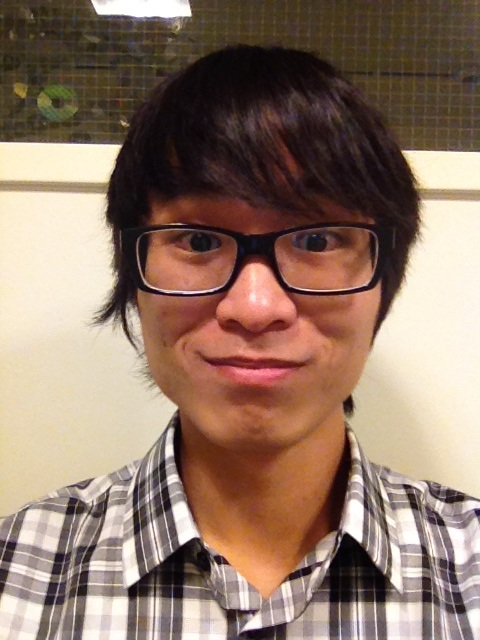
\includegraphics[height=8.0cm]{ek_headshot.jpg}
\caption{A recent photo of Eric.}
\end{figure}

\end{document}

